\documentclass[10pt]{beamer}
\usepackage[utf8]{inputenc}
\usepackage[T1]{fontenc}
\usepackage{lmodern}
\usepackage[catalan]{babel}
\usepackage{amsmath, amssymb}
\usepackage{graphicx}
\usepackage{tikz}
\usepackage{dirtytalk}

% Tema de la presentació
\usetheme{Madrid}
\usecolortheme{default}

% Informació del TFG
\title[Encabiments Isomètrics $C^1$]{Encabiments Isomètrics $C^1$ i $C^\infty$ en $\mathbb{R}^n$}
\author{Víctor Rubio Jiménez}
\institute{Universitat de Barcelona \\ Facultat de Matemàtiques i Informàtica}
\date{27 de juny de 2025}

% Comando per al supervisor
\newcommand{\supervisor}[1]{\def\insertsupervisor{{#1}}}
\supervisor{Dr. Ignasi Mundet i Riera}

% Definició de la pàgina de títol personalitzada
\makeatletter
\setbeamertemplate{title page}{
  \vbox{}
  \vfill
  \begingroup
    \centering
    \begin{beamercolorbox}[sep=8pt,center]{title}
      \usebeamerfont{title}\inserttitle\par%
      \ifx\insertsubtitle\@empty%
      \else%
        \vskip0.25em%
        {\usebeamerfont{subtitle}\usebeamercolor[fg]{subtitle}\insertsubtitle\par}%
      \fi%     
    \end{beamercolorbox}%
    \vskip1em\par
    \begin{beamercolorbox}[sep=8pt,center]{author}
      \usebeamerfont{author}\insertauthor
    \end{beamercolorbox}
    \begin{beamercolorbox}[sep=8pt,center]{institute}
      \usebeamerfont{institute}\insertinstitute
    \end{beamercolorbox}
    \begin{beamercolorbox}[sep=8pt,center]{author}
        \vspace{0.5cm}
      \usebeamerfont{small}Supervisor: \insertsupervisor
    \end{beamercolorbox}
    \begin{beamercolorbox}[sep=8pt,center]{date}
      \usebeamerfont{date}\insertdate
    \end{beamercolorbox}\vskip0.5em
  \endgroup
  \vfill
}
\makeatother


\begin{document}

% --- DIAPOSITIVA 1: Títol i Estructura ---
\begin{frame}
    \titlepage
\end{frame}

\begin{frame}
    \frametitle{Estructura de la presentació}
    \tableofcontents
\end{frame}

\section{Introducció a la Geometria Riemanniana}

\begin{frame}
    \frametitle{Introducció general}
    \begin{itemize}
        \item \textbf{Objectiu del treball:} Mostrar el guany en flexibilitat que suposa la regularitat $C^1$ en comparació amb la regularitat $C^\infty$ en el problema dels encabiments isomètrics.
        \pause
        \item \textbf{Estructura:}
        \begin{enumerate}
            \item Introducció als conceptes fonamentals.
            \pause
            \item La rigidesa dels encabiments $C^\infty$: exemples del tor pla i la cinta de Möbius.
            \pause
            \item La flexibilitat dels encabiments $C^1$: el teorema de Nash-Kuiper.
            \pause
            \item Una construcció explícita: l'encabiment $C^1$ del tor pla a $\mathbb{R}^3$.
        \end{enumerate}
    \end{itemize}
\end{frame}

\begin{frame}
  \frametitle{Conceptes fonamentals: varietats riemannianes}
  
  \begin{columns}[T] % L'opció [T] alinea les columnes per la part superior
      
      % Columna esquerra per al text
      \begin{column}{0.55\textwidth}
          
          % El bloc 1 és visible des del pas 1 en endavant
          \begin{block}<1->{Varietat Topològica}
              Un espai localment homeomorf a $\mathbb{R}^n$, Hausdorff i 2-numerable.
          \end{block}
          
          % El bloc 2 és visible des del pas 2 en endavant
          \begin{block}<2->{Varietat Diferenciable}
              Una varietat topològica a la qual afegim una estructura diferenciable, que ens permet fer càlcul (definir vectors tangents, derivades, etc.). Si és de classe $C^\infty$, l'anomenem \textbf{suau}.
          \end{block}
          
          % El bloc 3 és visible des del pas 3 en endavant
          \begin{block}<3->{Varietat Riemanniana}
              Una varietat diferenciable dotada d'una \textbf{mètrica riemanniana}. Aquesta mètrica assigna un producte escalar a l'espai tangent de cada punt, permetent mesurar longituds i angles de manera \textbf{intrínseca}.
          \end{block}
          
      \end{column}
      
      % Columna dreta per a les imatges
      \begin{column}{0.4\textwidth}
          \centering
          \vspace{2cm}
          
          % Imatge 1: Només visible al pas 1
          \only<1>{\vspace{1cm}\hspace{0.4cm}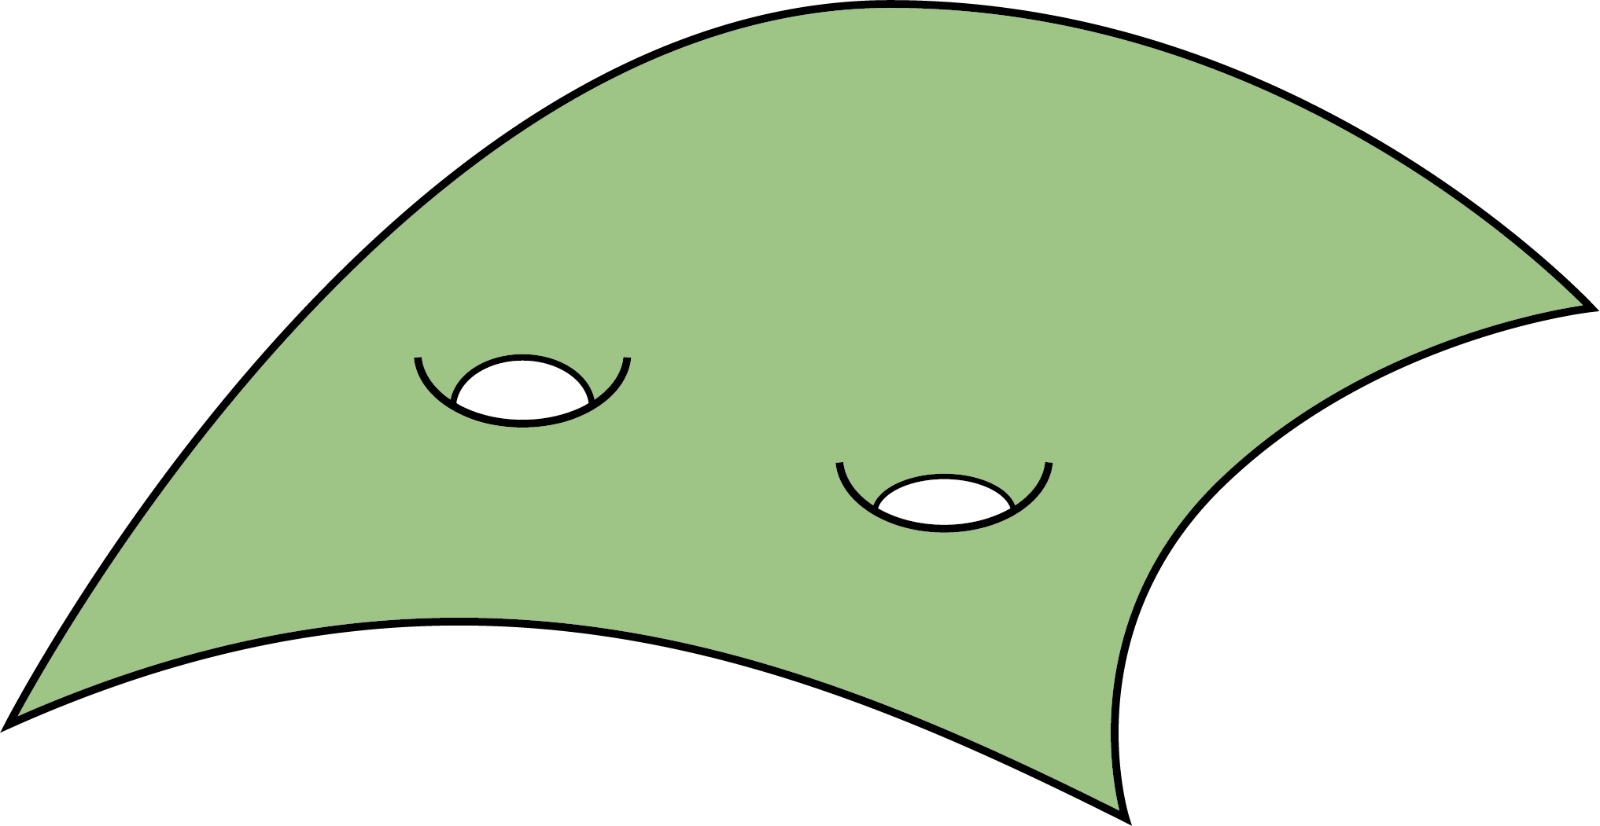
\includegraphics[width=\textwidth]{manifold.jpeg}}
          
          % Imatge 2: Només visible al pas 2
          \only<2>{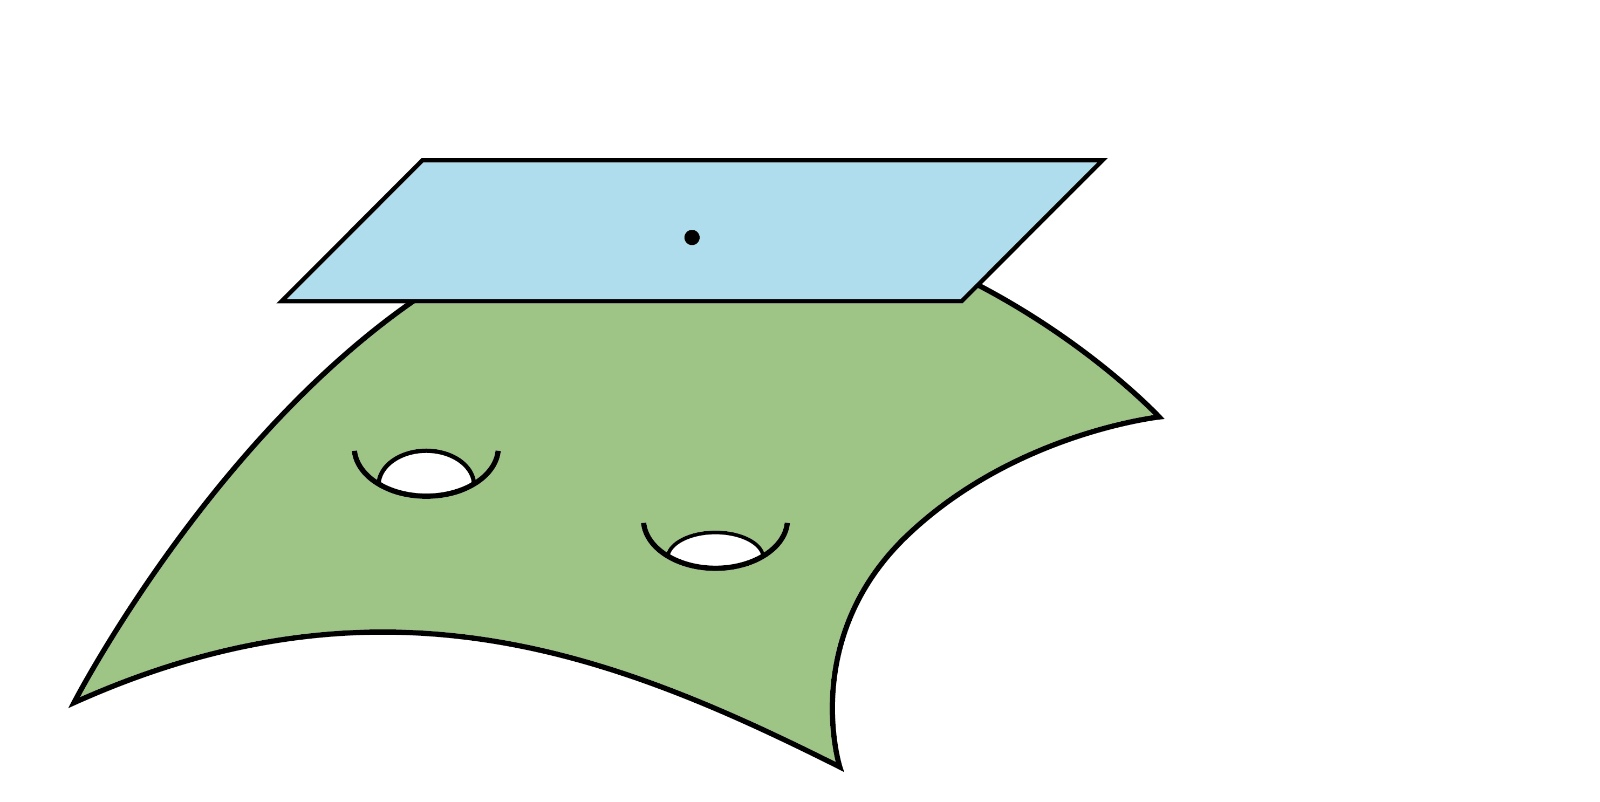
\includegraphics[width=1.5\textwidth]{tangent.jpeg}}
          
          % Imatge 3: Només visible al pas 3
          \only<3>{
            \begin{tikzpicture}
              \node (img) {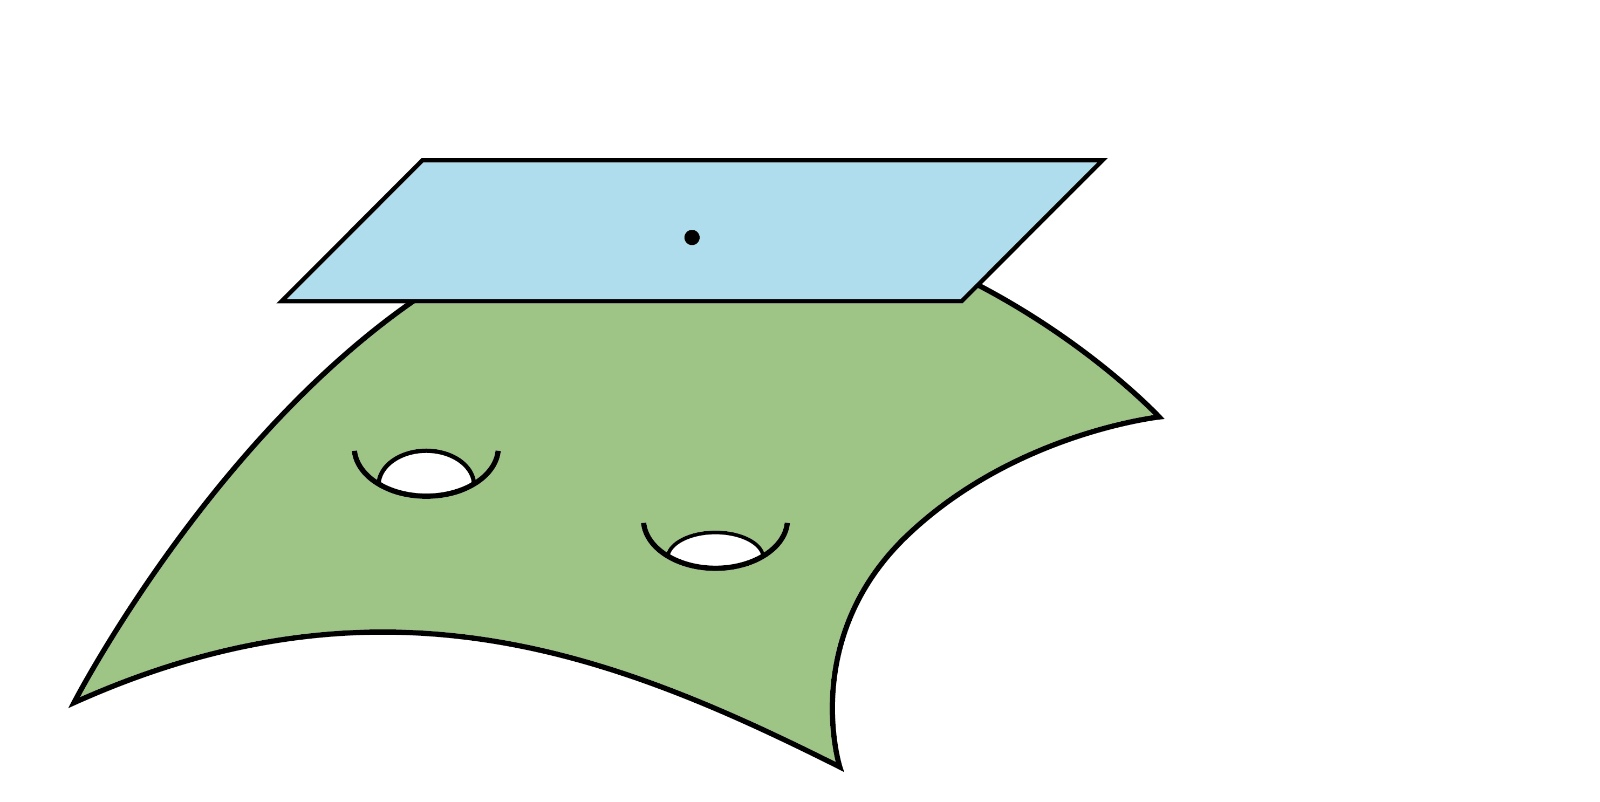
\includegraphics[width=1.5\textwidth]{tangent.jpeg}};
              \node[above=-1.5cm] at (img.north) {$g_{ij}$};
            \end{tikzpicture}
          }
          
      \end{column}
      
  \end{columns}
\end{frame}

\begin{frame}
    \frametitle{Encabiments i isometries}

    \begin{block}{Encabiment i Geometria Extrínseca}
        Un \textbf{encabiment} és una aplicació $C^k$ injectiva, homeomorfisme sobre la seva imatge i amb diferencial no singular.
        
        Si l'espai ambient té una mètrica, la varietat encabida hereta una \textbf{mètrica induïda}. Aquesta defineix la seva geometria \textbf{extrínseca}.
    \end{block}
    \pause
    
    \begin{block}{Encabiment Isomètric}
        Un encabiment és \textbf{isomètric} si preserva la mètrica: la geometria intrínseca de la varietat original coincideix amb la geometria extrínseca induïda per l'encabiment.
        
        \vspace{0.5cm}
        \centering
        \alert{Mètrica Intrínseca = Mètrica Induïda}
    \end{block}
    
\end{frame}

\begin{frame}
    \frametitle{La pregunta central}
    
    \begin{center}
        \LARGE
        Si una varietat riemanniana es pot encabir en algun espai euclidià $\mathbb{R}^N$, es pot encabir isomètricament?
    \end{center}
    
    \pause
    
    \begin{columns}
        \begin{column}{0.5\textwidth}
            \begin{block}{El cas $C^\infty$}
                \textbf{Teorema de Whitney:} Tota varietat suau n-dimensional es pot encabir en $\mathbb{R}^{2n+1}$.
                \vspace{0.3cm}
                
                \alert{Però no garanteix que sigui isomètric!} La curvatura i altres nocions poden imposar restriccions molt fortes.
            \end{block}
        \end{column}
        \begin{column}{0.5\textwidth}
            \begin{block}{El cas $C^1$}
                \textbf{Resposta (Spoiler):} \textit{Sí! } Sempre és possible trobar un encabiment isomètric $C^1$.
                 \vspace{0.3cm}
                
                La regularitat $C^1$ és molt més flexible i permet \say{esquivar} les restriccions del cas suau.
            \end{block}
        \end{column}
    \end{columns}
    
\end{frame}

\section{La Rigidesa dels Encabiments $C^\infty$}

\begin{frame}
    \frametitle{El tor pla: un exemple de rigidesa $C^\infty$}

    \begin{block}{Definició}
        Un \textbf{tor} és una varietat topològica que resulta d'identificar els costats oposats d'un rectangle.
        
        Un \textbf{tor pla} és un tor dotat de la mètrica euclidiana plana.
    \end{block}
    
    \begin{figure}
        % TODO: Reemplaça amb una imatge de la construcció del tor
        \includegraphics[height=3cm]{tor_identificat.pdf}
      \includegraphics[height=3cm]{torcosa.pdf}
      \caption{Identificació dels costats d'un quadrat per formar un tor (esquerra) i encabiment d'un tor pla en $\mathbb{R}^3$ (dreta).}
  \end{figure}
  
    
\end{frame}

\begin{frame}
    \frametitle{La impossibilitat d'encabir el tor pla en $\mathbb{R}^3$}
    
    \begin{block}{Argument de la Demostració}
        \begin{itemize}
            \item \textbf{Teorema 1:} Tota superfície compacta, suau ($C^\infty$) i encabida en $\mathbb{R}^3$ ha de tenir punts de \textbf{curvatura Gaussiana positiva}.
            \pause
            \item \textbf{Teorema 2 (Egregi de Gauss):} La curvatura Gaussiana és una noció \textbf{intrínseca}. Un encabiment isomètric ha de conservar-la.
            \pause
            \item \textbf{Contradicció:}
            \begin{enumerate}
                \item Si un tor pla s'encabís isomètricament i $C^\infty$ en $\mathbb{R}^3$, hauria de tenir punts de curvatura positiva (per ser compacte).
                \item Però, per ser isomètric al tor pla, la seva curvatura hauria de ser zero a tot arreu.
            \end{enumerate}
            \pause
            \Large \centering \alert{Conclusió: És impossible!}
        \end{itemize}
    \end{block}
    
\end{frame}

\begin{frame}
    \frametitle{Un altre exemple: la cinta de Möbius}
    
    \begin{block}{Cinta de Möbius de Paper}
        S'obté identificant dos costats oposats d'un rectangle de costats $1$ i $\lambda$, però invertint l'orientació.
        \begin{itemize}
            \item La \textbf{raó d'aspecte} és $\lambda$.
            \item Una \textbf{cinta de Möbius de paper} és un encabiment isomètric i $C^\infty$ d'aquesta varietat en $\mathbb{R}^3$.
        \end{itemize}
    \end{block}

    \begin{figure}
        \centering
        \includegraphics[width=0.4\textwidth]{cinta.pdf}
        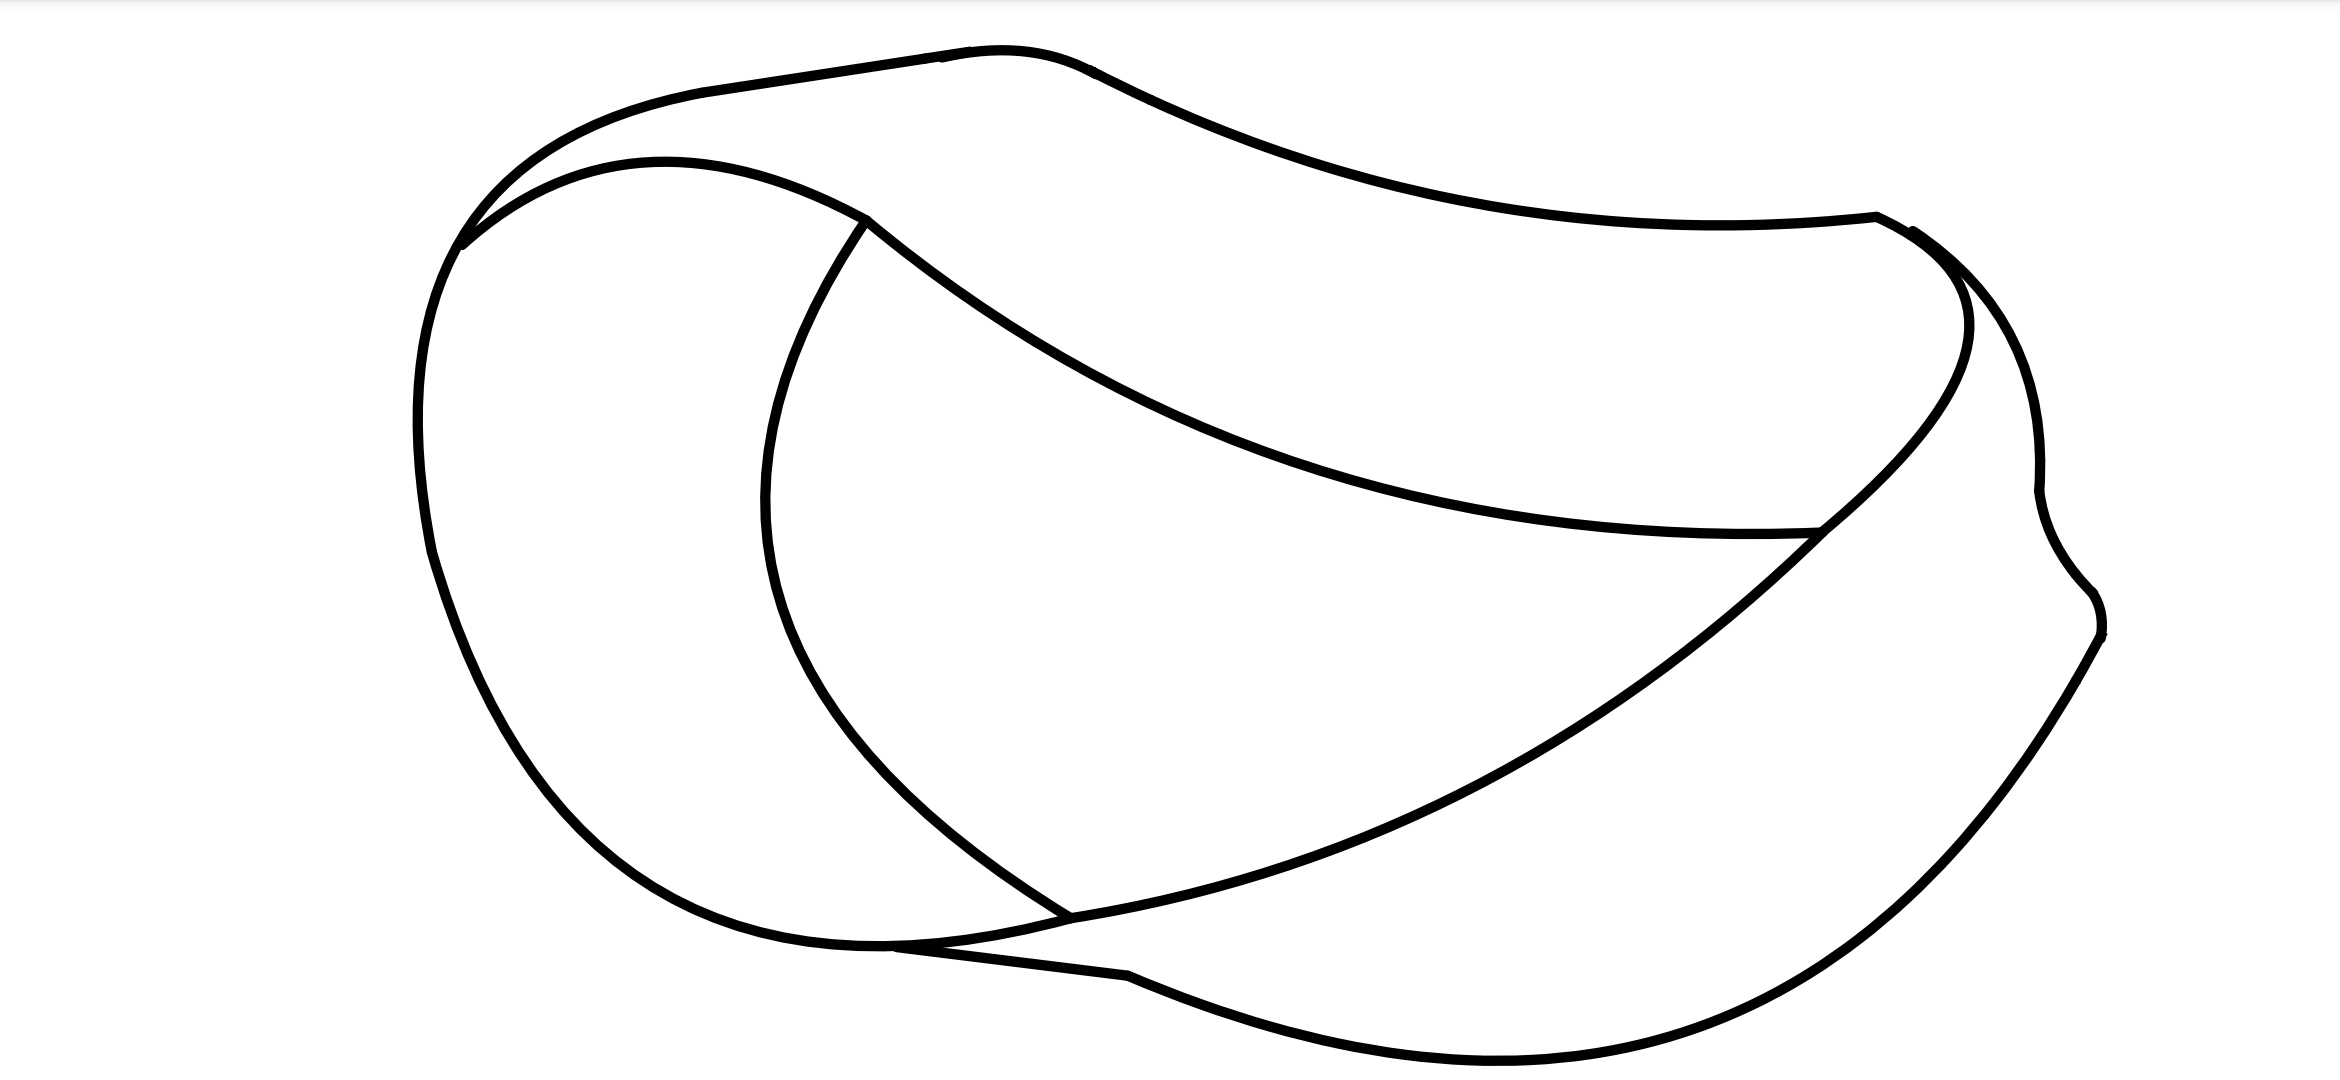
\includegraphics[width=0.4\textwidth]{encabida.jpg}
        \caption{Cinta de Möbius plana (esquerra) i encabiment d'una cinta de Möbius en $\mathbb{R}^3$ (dreta).}
    \end{figure}
    
\end{frame}

\begin{frame}
    \frametitle{El Teorema de Schwartz}

    \begin{block}{Un Resultat Recent (2024)}
        Richard Evan Schwartz va demostrar que:
        \vspace{0.5cm}
        \begin{center}
            \textit{Qualsevol cinta de Möbius de paper encabida en $\mathbb{R}^3$ ha de tenir una raó d'aspecte $\lambda > \sqrt{3}$.}
        \end{center}
        \vspace{0.5cm}
        Això és un altre teorema d'impossibilitat: si una cinta és massa \say{curta i ampla}, no es pot encabir isomètricament i de manera suau.
    \end{block}
    
    \begin{figure}
        \centering
        \includegraphics[width=0.25\textwidth]{cinta_triangular.pdf}
        \caption{Cinta de Möbius plana més petita que es pot encabir isomètricament i de manera suau.}
    \end{figure}
    
\end{frame}

\begin{frame}
    \frametitle{L'obstacle comú: la curvatura}
    
    \begin{block}{Què uneix aquests dos exemples?}
        En ambdós casos, l'obstacle per a un encabiment isomètric $C^\infty$ és la \textbf{curvatura}.
        \begin{itemize}
            \item \textbf{Tor Pla:} La curvatura de Gauss hauria de ser 0 i positiva alhora.
            \pause
            \item \textbf{Cinta de Möbius:} La demostració de Schwartz es basa en l'existència d'una foliació per segments de recta (plecs), la qual depèn d'arguments sobre la \textbf{curvatura mitjana} de la superfície.
        \end{itemize}
    \end{block}
    \pause
    \begin{alertblock}{La Clau}
        Aquestes nocions de curvatura (Gaussiana, mitjana) requereixen que l'encabiment sigui com a mínim de classe $C^2$. Si la regularitat és menor, aquestes restriccions desapareixen.
    \end{alertblock}
    
\end{frame}

\begin{frame}
    \frametitle{Esquivant la rigidesa: l'acordió de Möbius}

    \begin{block}{Un \say{contraexemple} visual}
        Prenem un paper quadrat ($\lambda=1 < \sqrt{3}$). Segons el teorema de Schwartz, no es pot encabir isomètricament i $C^\infty$.
        
        Però podem fer això:
    \end{block}
    
      \begin{figure}
          % TODO: Reemplaçar amb una seqüència d'imatges de l'acordió de Möbius.
          \centering
          \fbox{\includegraphics[width=0.2\textwidth]{acordió.pdf}}
      \end{figure}
    \pause
    
    \begin{alertblock}{Com és possible?}
        En els doblecs, la curvatura no està ben definida. L'encabiment no és $C^\infty$, ni tan sols $C^1$. És un encabiment $C^\infty$ a trossos.
        
        \textbf{Conclusió:} Baixant la regularitat, guanyem flexibilitat. Podem fer-ho de manera més controlada, per exemple, aconseguint un encabiment $C^1$?
    \end{alertblock}

\end{frame}


\section{El Teorema de Nash-Kuiper}

\begin{frame}
    \frametitle{El trencament $C^1$: el Teorema de Nash (1954)}

    \begin{block}{Enunciat del Teorema}
        Qualsevol encabiment $C^\infty$ \textbf{curt} d'una varietat riemanniana n-dimensional en $\mathbb{R}^{n+k}$ (amb $k \geq 2$) es pot aproximar per un encabiment \textbf{isomètric} de classe \textbf{$C^1$}, arbitràriament proper a l'original.
    \end{block}
    
    \begin{itemize}
        \item A més, sempre existeix algun encabiment $C^\infty$ curt en $\mathbb R^{2n+1}$.
        \pause
        \item Aquest resultat implica que \textbf{qualsevol varietat riemanniana} admet un encabiment isomètric $C^1$ en algun espai euclidià.
    \end{itemize}
    
\end{frame}

\begin{frame}
    \frametitle{Esbós de la demostració de Nash (I)}
    
    \textbf{Organització general}
    \begin{itemize}
        \item $f:M \to \mathbb{R}^N$ de classe $C^\infty$ curt.
        \item El procés es divideix en \textbf{etapes}, cadascuna de les quals es divideix en \textbf{passos}.
        \item Cada pas afegeix una pertorbació en una regió de la varietat.
        \item Després de cada etapa, s'obté un encabiment $C^\infty$ que és menys curt que l'anterior.
    \end{itemize}
\end{frame}

\begin{frame}
    \frametitle{Esbós de la demostració de Nash (II)}
    
    \textbf{El punt de partida}
    \begin{itemize}
        \item Sigui $f:M \to \mathbb{R}^N$ de classe $C^\infty$.
        \item La mètrica induïda en la imatge és $h_{ij} = \sum_{\alpha} \frac{\partial z^\alpha}{\partial x^i}\frac{\partial z^\alpha}{\partial x^j}$.
        \item Si $f$ és curt, aleshores $g_{ij}(u,v) \ge h_{ij}(D_pf(u),D_pf(v))$ per a tot $u,v \in T_pM$
        \item {Sempre és possible trobar un encabiment d'aquesta mena.}
    \end{itemize}
\end{frame}

\begin{frame}
    \frametitle{Esbós de la demostració de Nash (III)}
    
    \textbf{La partició}
    \begin{itemize}
        \item Dividim $M$ en entorns $N_p$ compactes.
        \item Per cada $N_p$, tenim una funció suau $\varphi_p: M \to \mathbb{R}_+$ tal que $\sum_p \varphi_p(x)=1$ per tot $x\in M$.
        \item POSAR UN DIBUIX.
    \end{itemize}
\end{frame}

\begin{frame}
    \frametitle{Esbós de la demostració de Nash (IV)}
    
    \textbf{L'error mètric}
    \begin{itemize}
        \item Anomenem error mètric $\delta_{ij} = g_{ij} - h_{ij}$.
        \item Per tot tensor $C^\infty$ definit positiu $\beta_{ij}$ sobre un entorn $N_p$ es pot trobar una descomposició finita de la forma següent:
        \begin{equation*}
            \frac12\varphi_p\beta_{ij} = \sum_\nu a_\nu \left(\frac{\partial\psi^\nu}{\partial x^i}\right)\left(\frac{\partial\psi^\nu}{\partial x^j}\right).
        \end{equation*}
    \end{itemize}
\end{frame}

\begin{frame}
    \frametitle{Esbós de la demostració de Nash (V)}
    
    \textbf{La pertorbació}
    \begin{itemize}
        \item Per cada entorn $N_p$, i per cada terme $\nu$ del sumatori, definim una pertorbació 
        \begin{equation*}
            \boxed{
            \overline{z}^\alpha = z^\alpha + \zeta^\alpha\frac{\sqrt{a_\nu}}{\lambda}\cos(\lambda \psi^\nu) + \eta^\alpha\frac{\sqrt{a_\nu}}{\lambda}\sin(\lambda \psi^\nu)}
        \end{equation*}
    \end{itemize}
    \begin{itemize}
        \item $\zeta, \eta$: Dos camps vectorials normals a la superfície. \alert{Això exigeix codimensió $\ge 2$!}
        \item $a_\nu$: L'amplitud de l'oscil·lació, relacionada amb l'error mètric a corregir.
        \item $\lambda$: La freqüència de l'oscil·lació, que podem fer tan gran com vulguem.
    \end{itemize}
\end{frame}

\begin{frame}
    \frametitle{Esbós de la demostració de Nash (VI)}
    
    \textbf{L'efecte de la pertorbació}
    \begin{itemize}
        \item La pertorbació disminueix l'error mètric en $N_p$ per aproximadament un terme del sumatori, $$a_\nu\frac{\partial\psi^\nu}{\partial x^i}\frac{\partial\psi^\nu}{\partial x^j},$$ de manera que deprés de realitzar un nombre finit de passos en $N_p$ hem augmentat la mètrica per $\frac12\varphi_p\beta_{ij}$.
        \item Hi ha un error d'ordre $O(1/\lambda)$ que podem controlar canviant $\lambda$.
        \item El canvi acumulat per les pertorbacions en les primeres derivades és menor que $2\sqrt{K\beta_{ii}}$ on $K$ és una constant que només depèn de la dimensió de la varietat.
    \end{itemize}
\end{frame}

\begin{frame}
    \frametitle{Esbós de la demostració de Nash (VII)}
    
    \textbf{El límit}
    \begin{itemize}
        \item Després de cada etapa, l'error mètric es divideix a la meitat.
        \item A més, les primeres derivades de l'encabiment convergeixen uniformement.
        \item Per tant, després d'infinites etapes, obtenim un encabiment isomètric i $C^1$ que és arbitràriament proper a l'encabiment inicial.
    \end{itemize}
\end{frame}

\begin{frame}
    \frametitle{El refinament de Kuiper (1955)}
    
    \begin{block}{La millora clau}
        El requisit de Nash de codimensió 2 era una limitació, especialment per a superfícies que volíem encabir a $\mathbb{R}^3$.
        
        Un any després, Nicolaas Kuiper va demostrar la conjectura de Nash: el resultat és cert per a \textbf{codimensió 1}.
    \end{block}
    \pause
    
    \begin{block}{La corrugació (\textit{Strain})}
        Kuiper va idear una pertorbació més sofisticada, una \textbf{corrugació}, que només necessita una direcció normal ($\eta^\beta$).
        \begin{equation*}
            \boxed{
                \overline{z}^\beta = z^\beta - \left(\frac{\overline \alpha^2}{8\lambda}\right)h\sin\left(2\lambda x^1\right)\xi^\beta + \left(\frac{\overline\alpha}{\lambda}\right)\sin\left(\lambda x^1 - \dots\right)h\eta^\beta
            }
        \end{equation*}
        Aquesta pertorbació compensa el moviment en la direcció normal $\eta$ amb un moviment en una direcció tangent $\xi$.
    \end{block}

\end{frame}

\section{Construcció d'un Encabiment Isomètric del Tor Pla}

\begin{frame}
    \frametitle{El tor pla en $\mathbb{R}^3$}
    
    \begin{itemize}
            \item Hem vist que un encabiment isomètric $C^\infty$ del tor pla en $\mathbb{R}^3$ és impossible.
            \item Però amb el teorema de Nash-Kuiper ($n=2, k=1 \implies N=3$), sabem que un encabiment isomètric \textbf{$C^1$ ha d'existir}!
        \end{itemize}
    \pause
    
    \begin{block}{Borrelli et al. (2013)}
        Realització d'un procés iteratiu concret per a trobar un encabiment isomètric $C^1$ del tor pla en $\mathbb{R}^3$ i dibuixar-lo amb ordinador.
    \end{block}
\end{frame}

\begin{frame}

    \begin{figure}
        \centering
        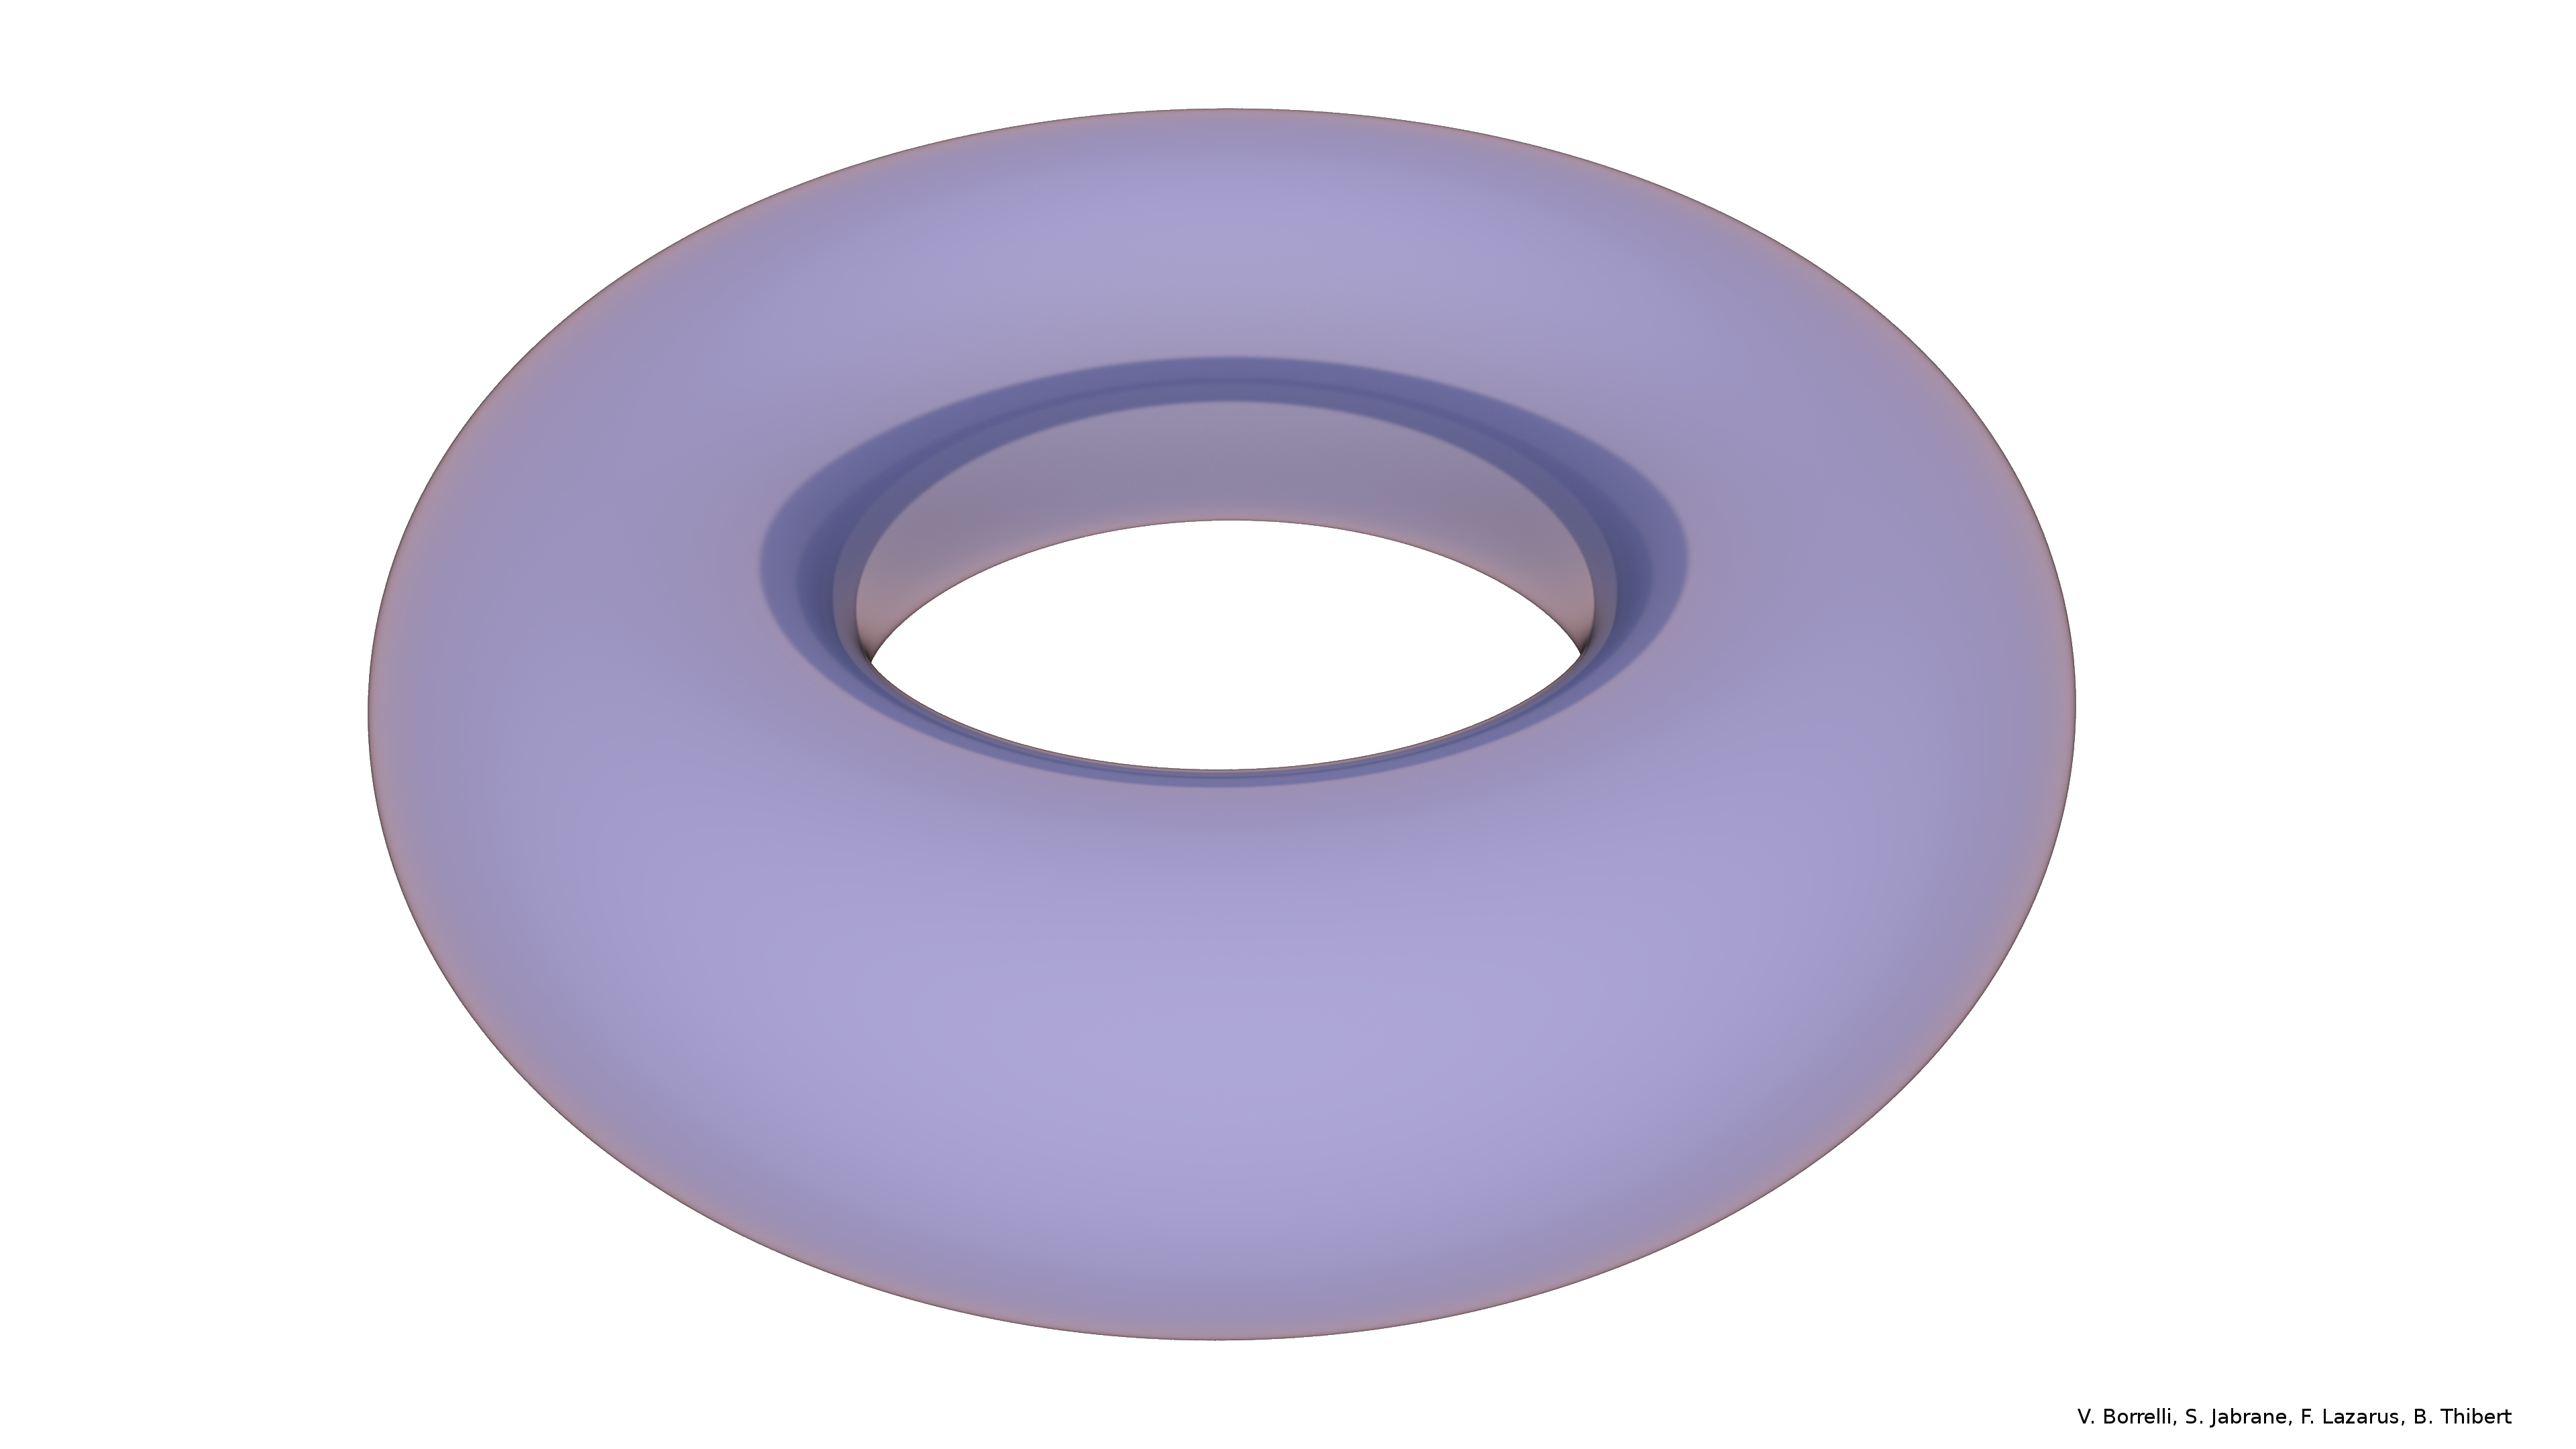
\includegraphics[width=0.8\textwidth]{0corrugation.jpg} % Nom de la imatge del tor
    \end{figure}
    
\end{frame}
\begin{frame}

    \begin{figure}
        \centering
        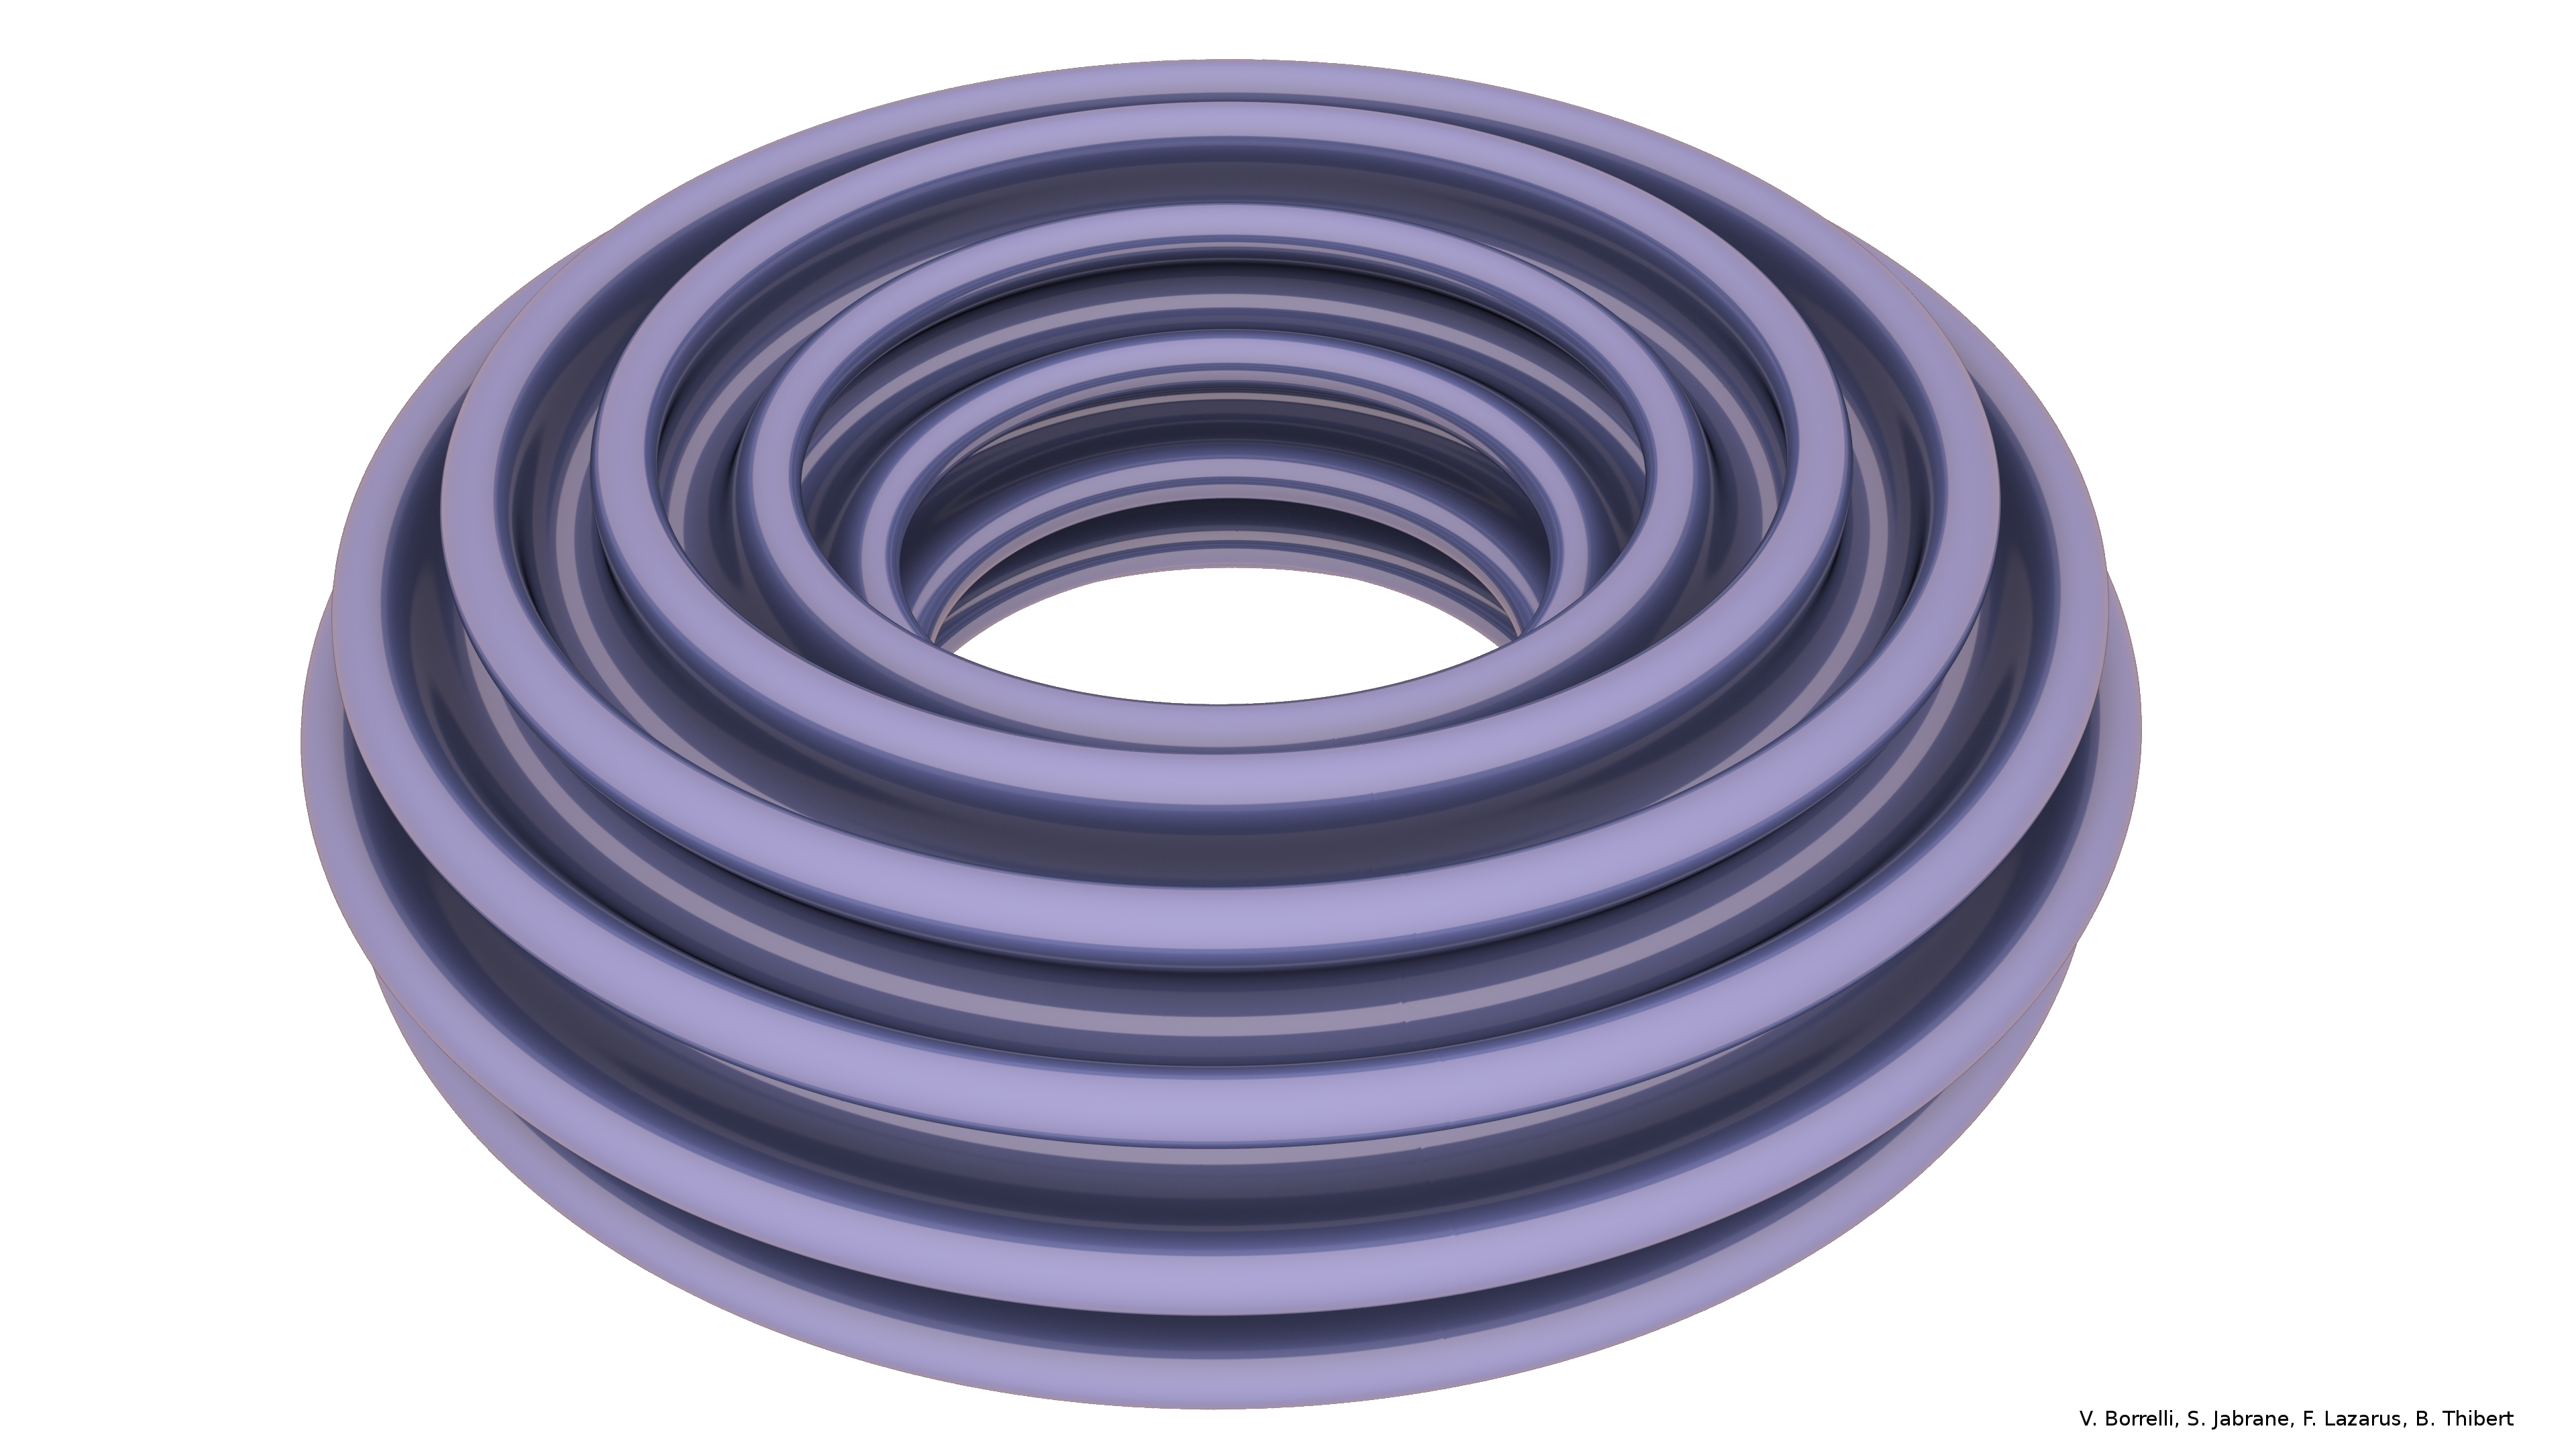
\includegraphics[width=0.8\textwidth]{1corrugation.jpg} % Nom de la imatge del tor
    \end{figure}
    
\end{frame}
\begin{frame}

    \begin{figure}
        \centering
        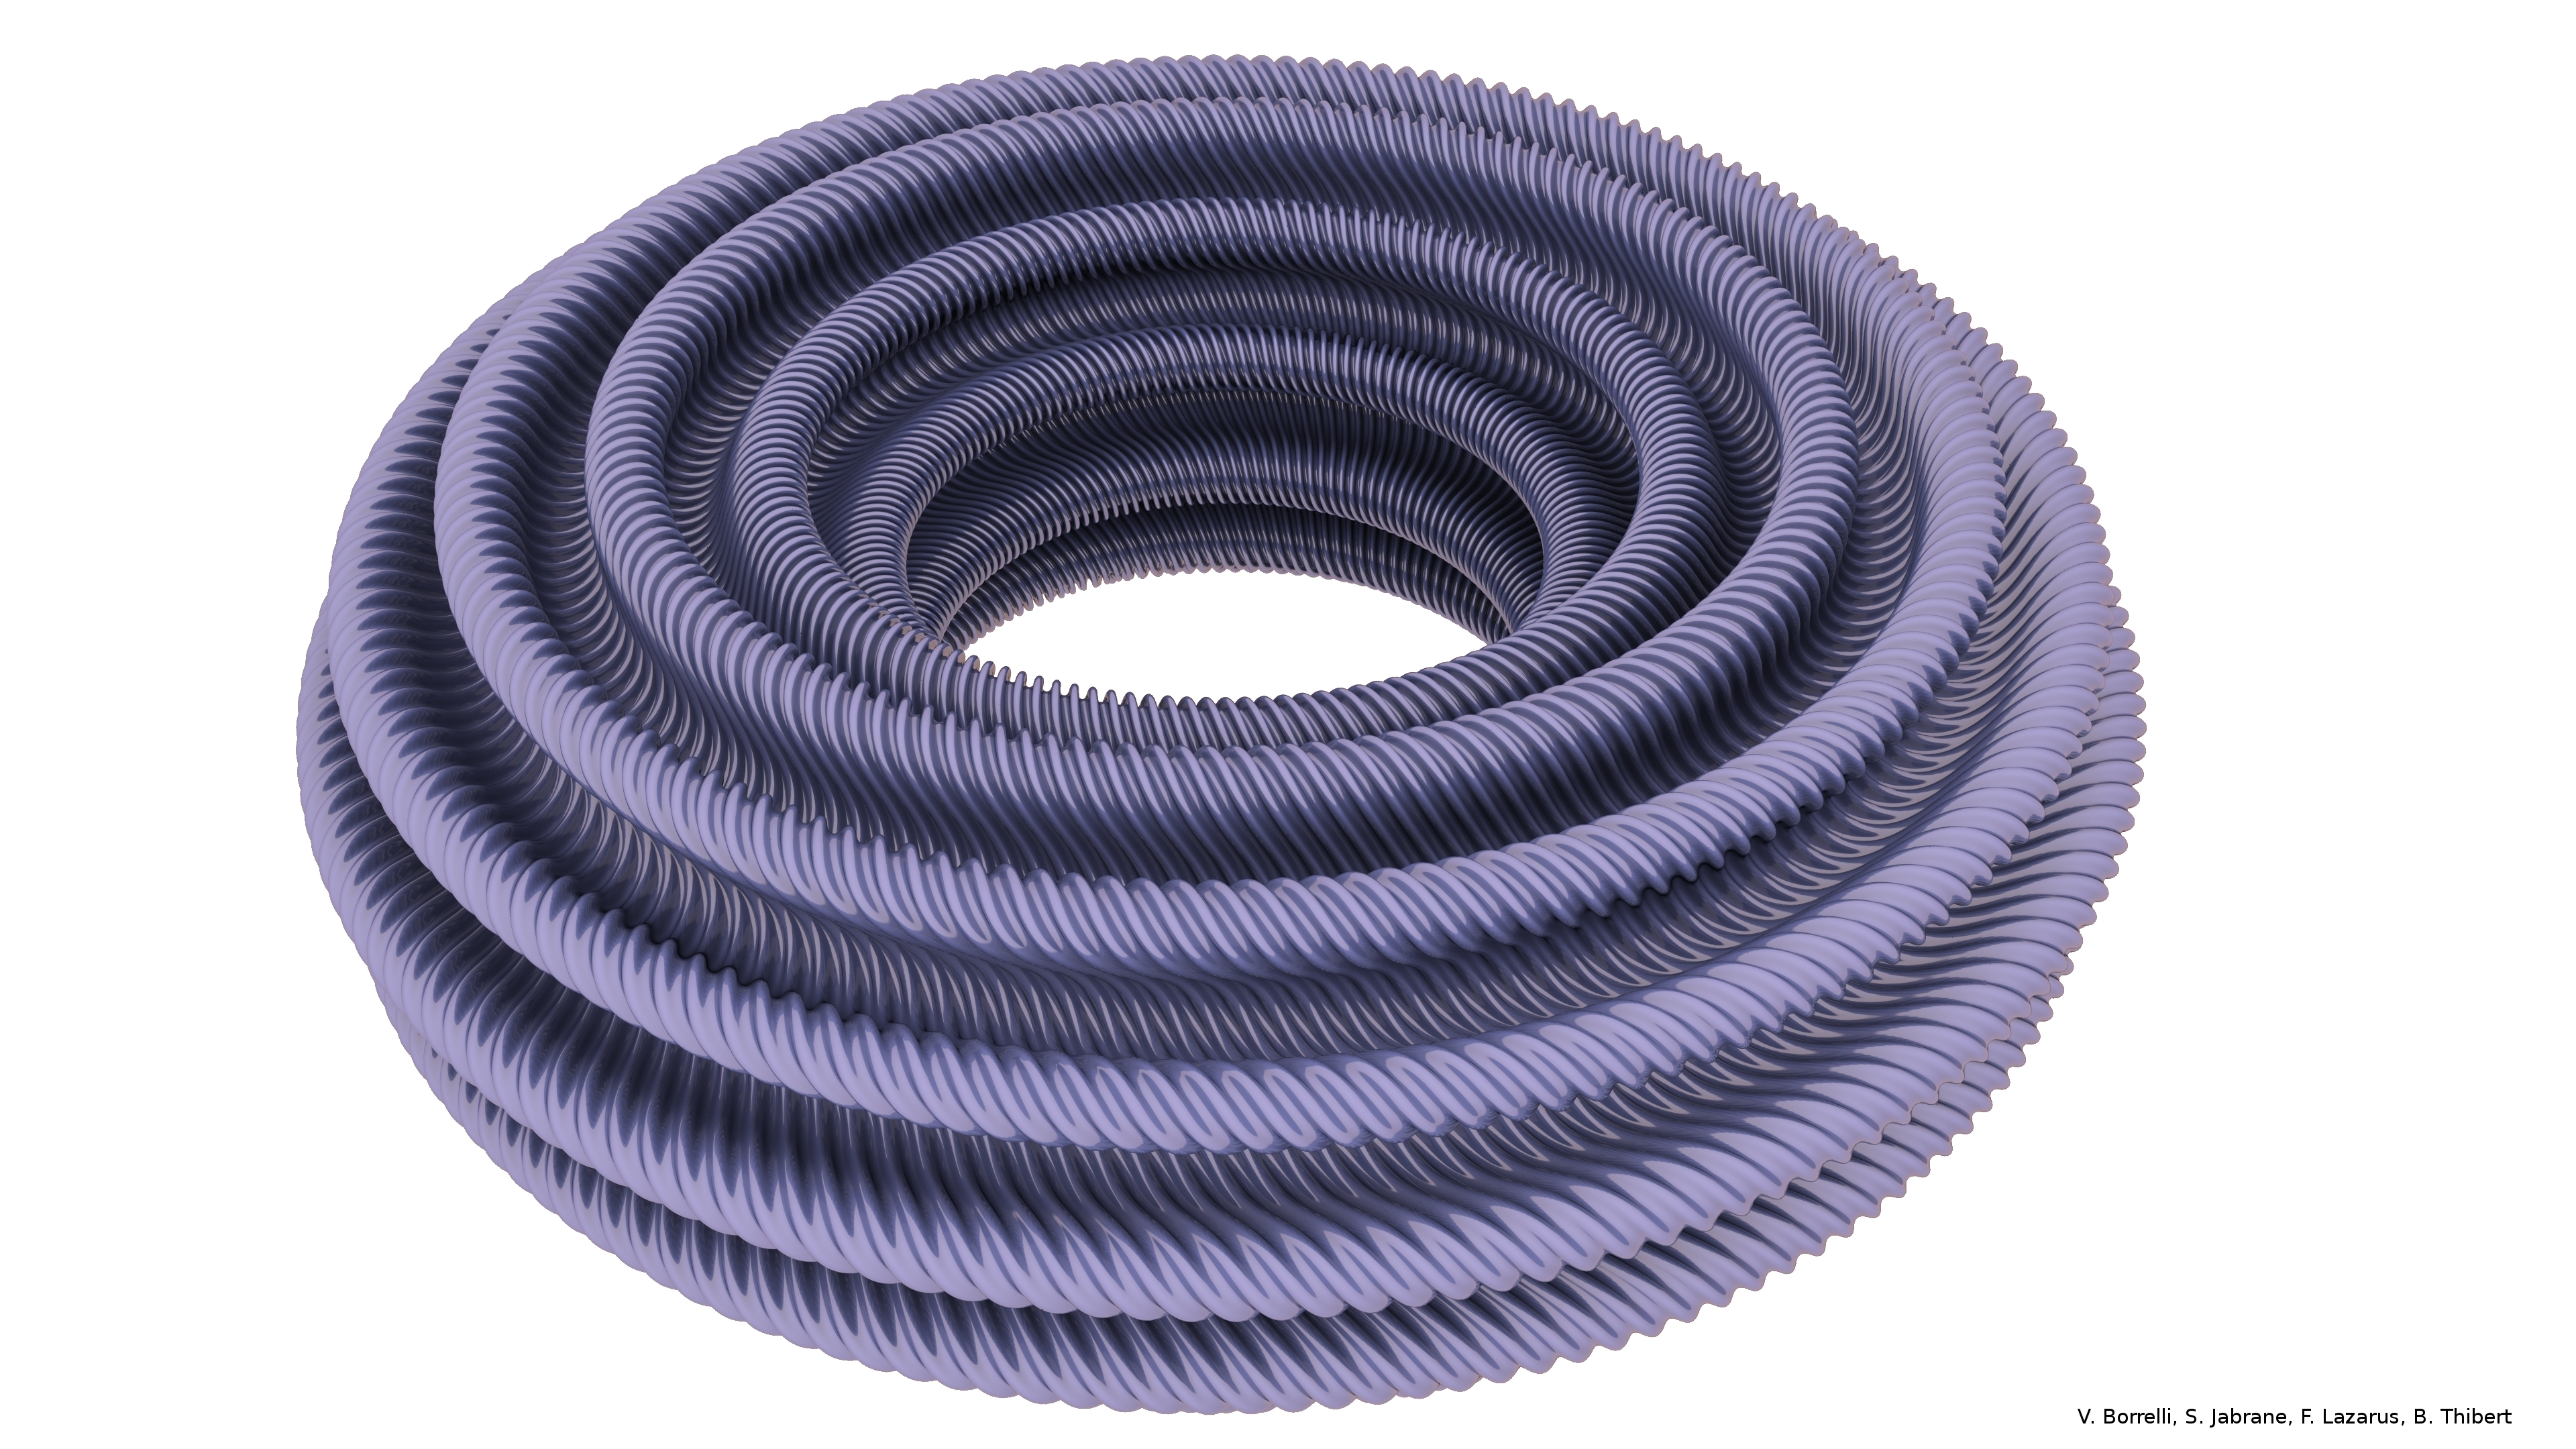
\includegraphics[width=0.8\textwidth]{2corrugations.jpg} % Nom de la imatge del tor
    \end{figure}
    
\end{frame}
\begin{frame}

    \begin{figure}
        \centering
        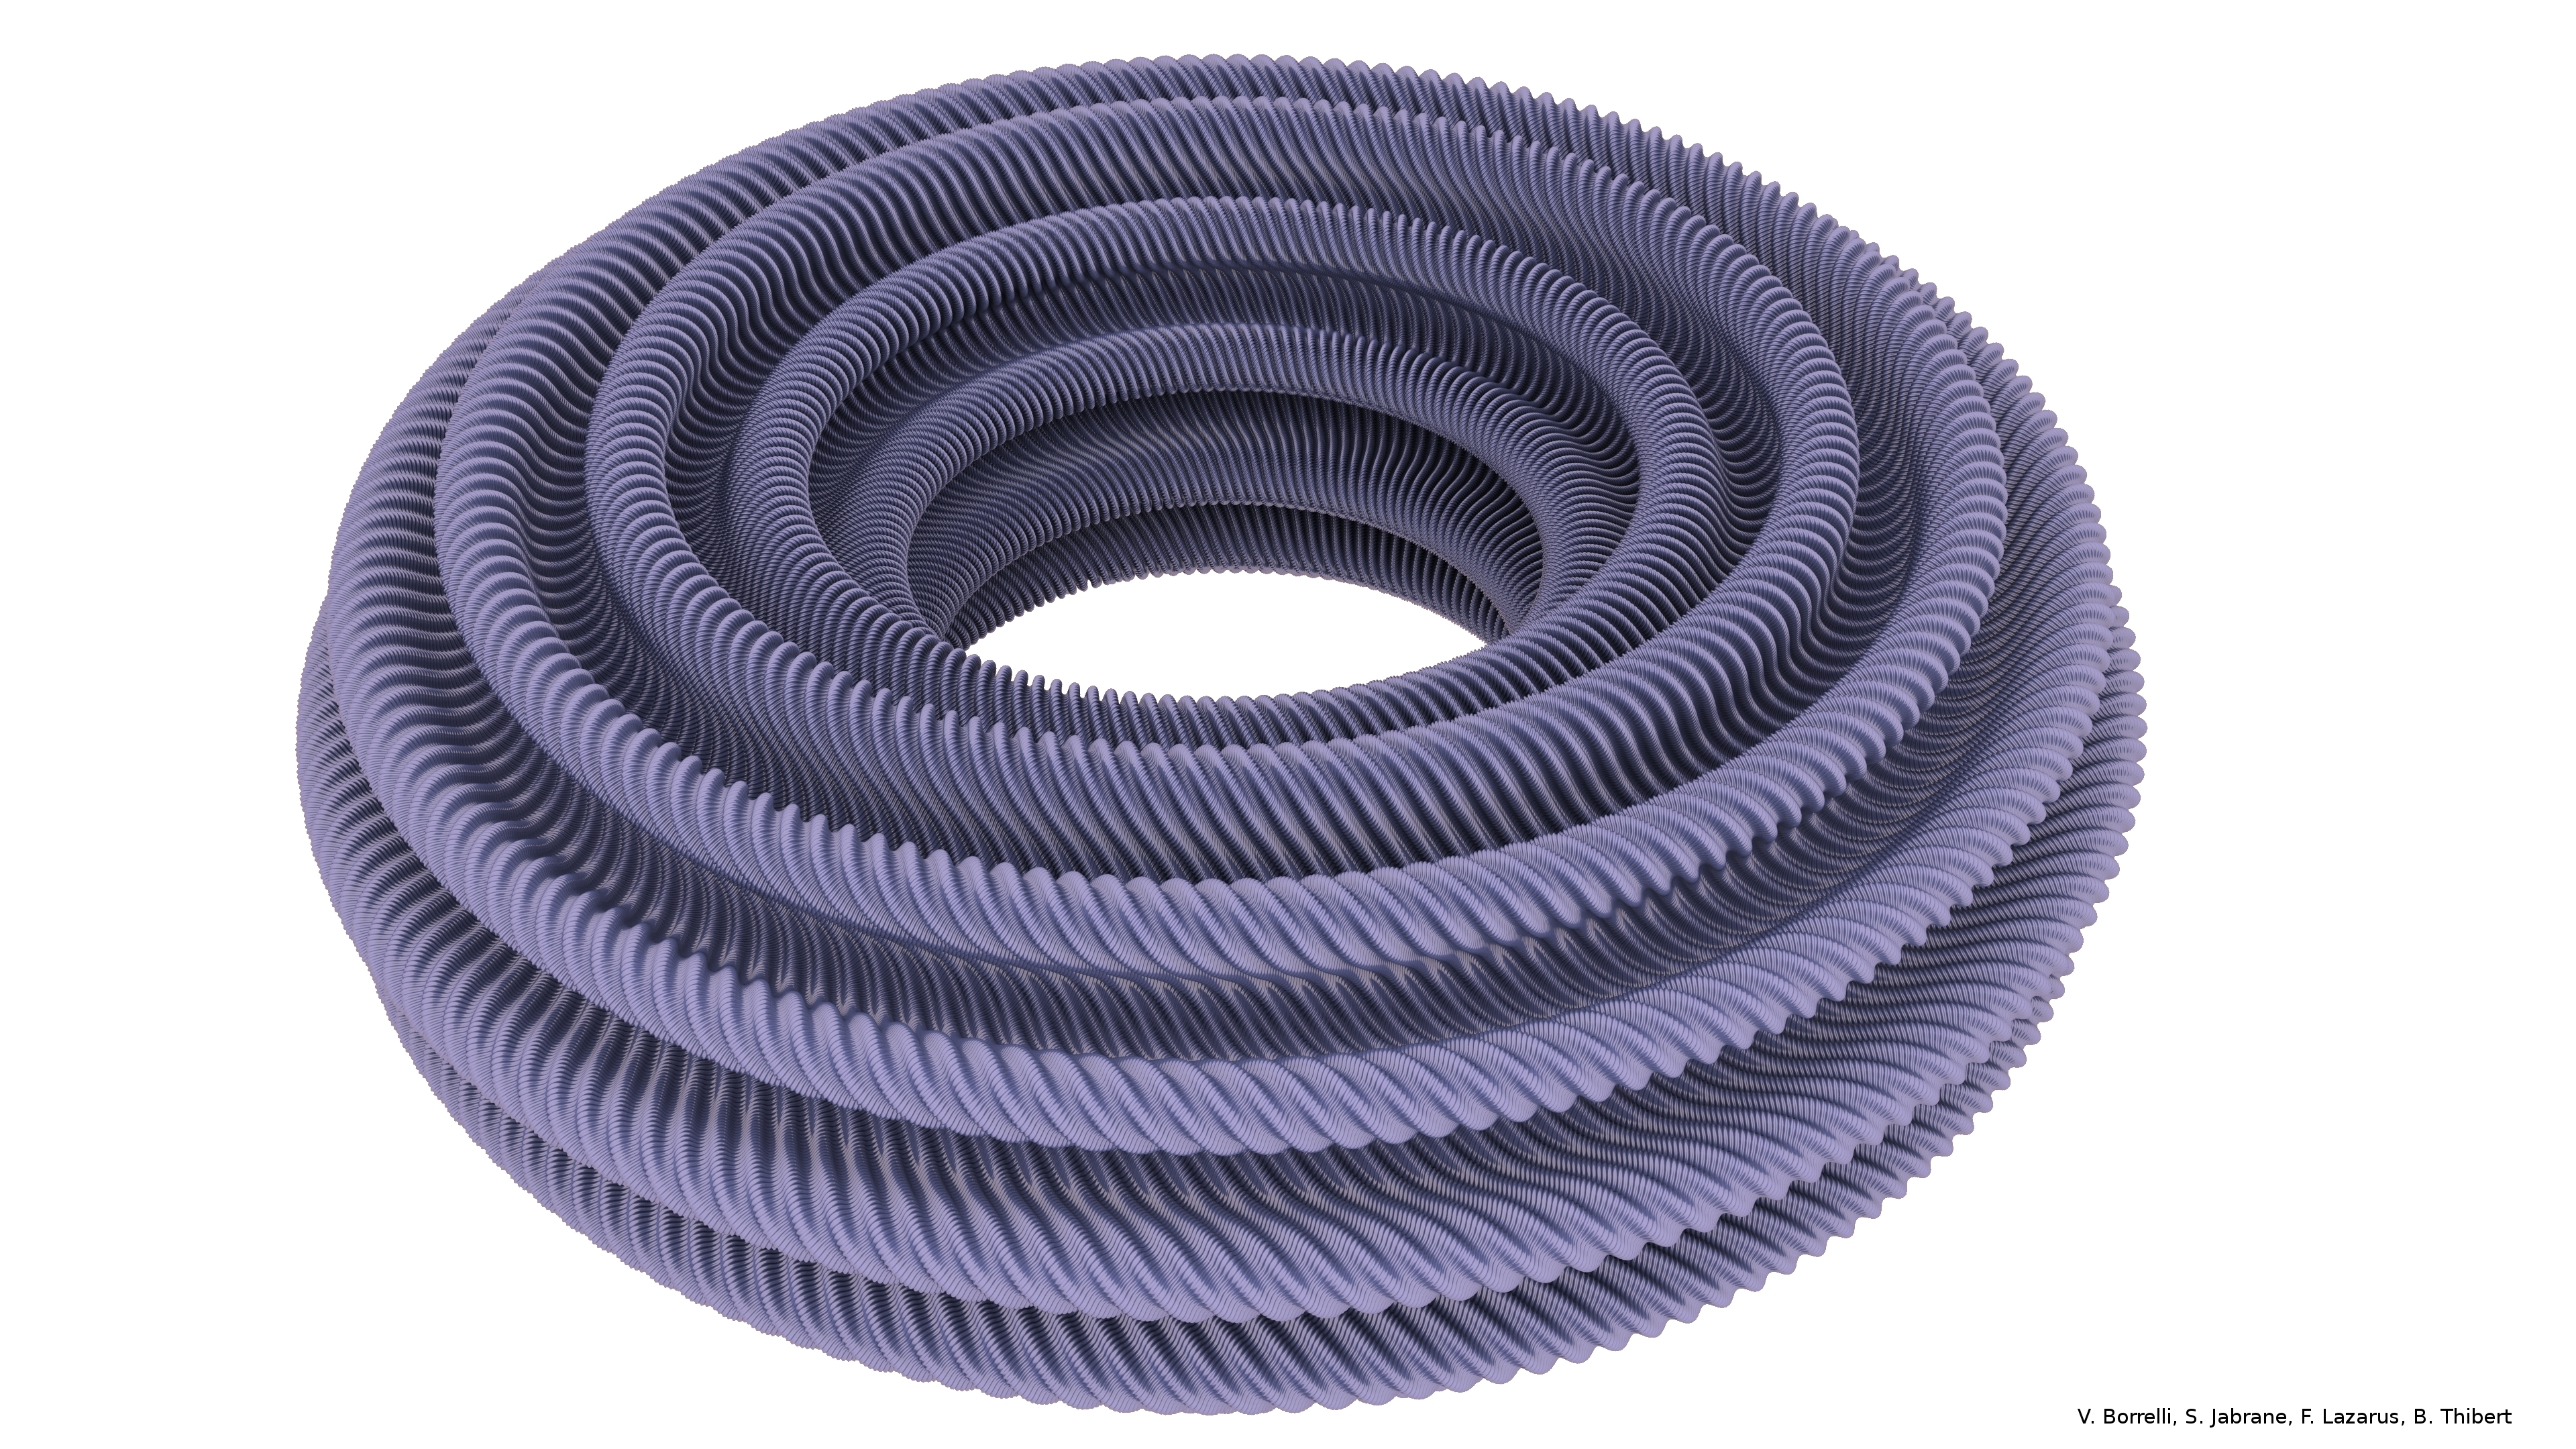
\includegraphics[width=0.8\textwidth]{3corrugations.jpg} % Nom de la imatge del tor
    \end{figure}
    
\end{frame}
\begin{frame}

    \begin{figure}
        \centering
        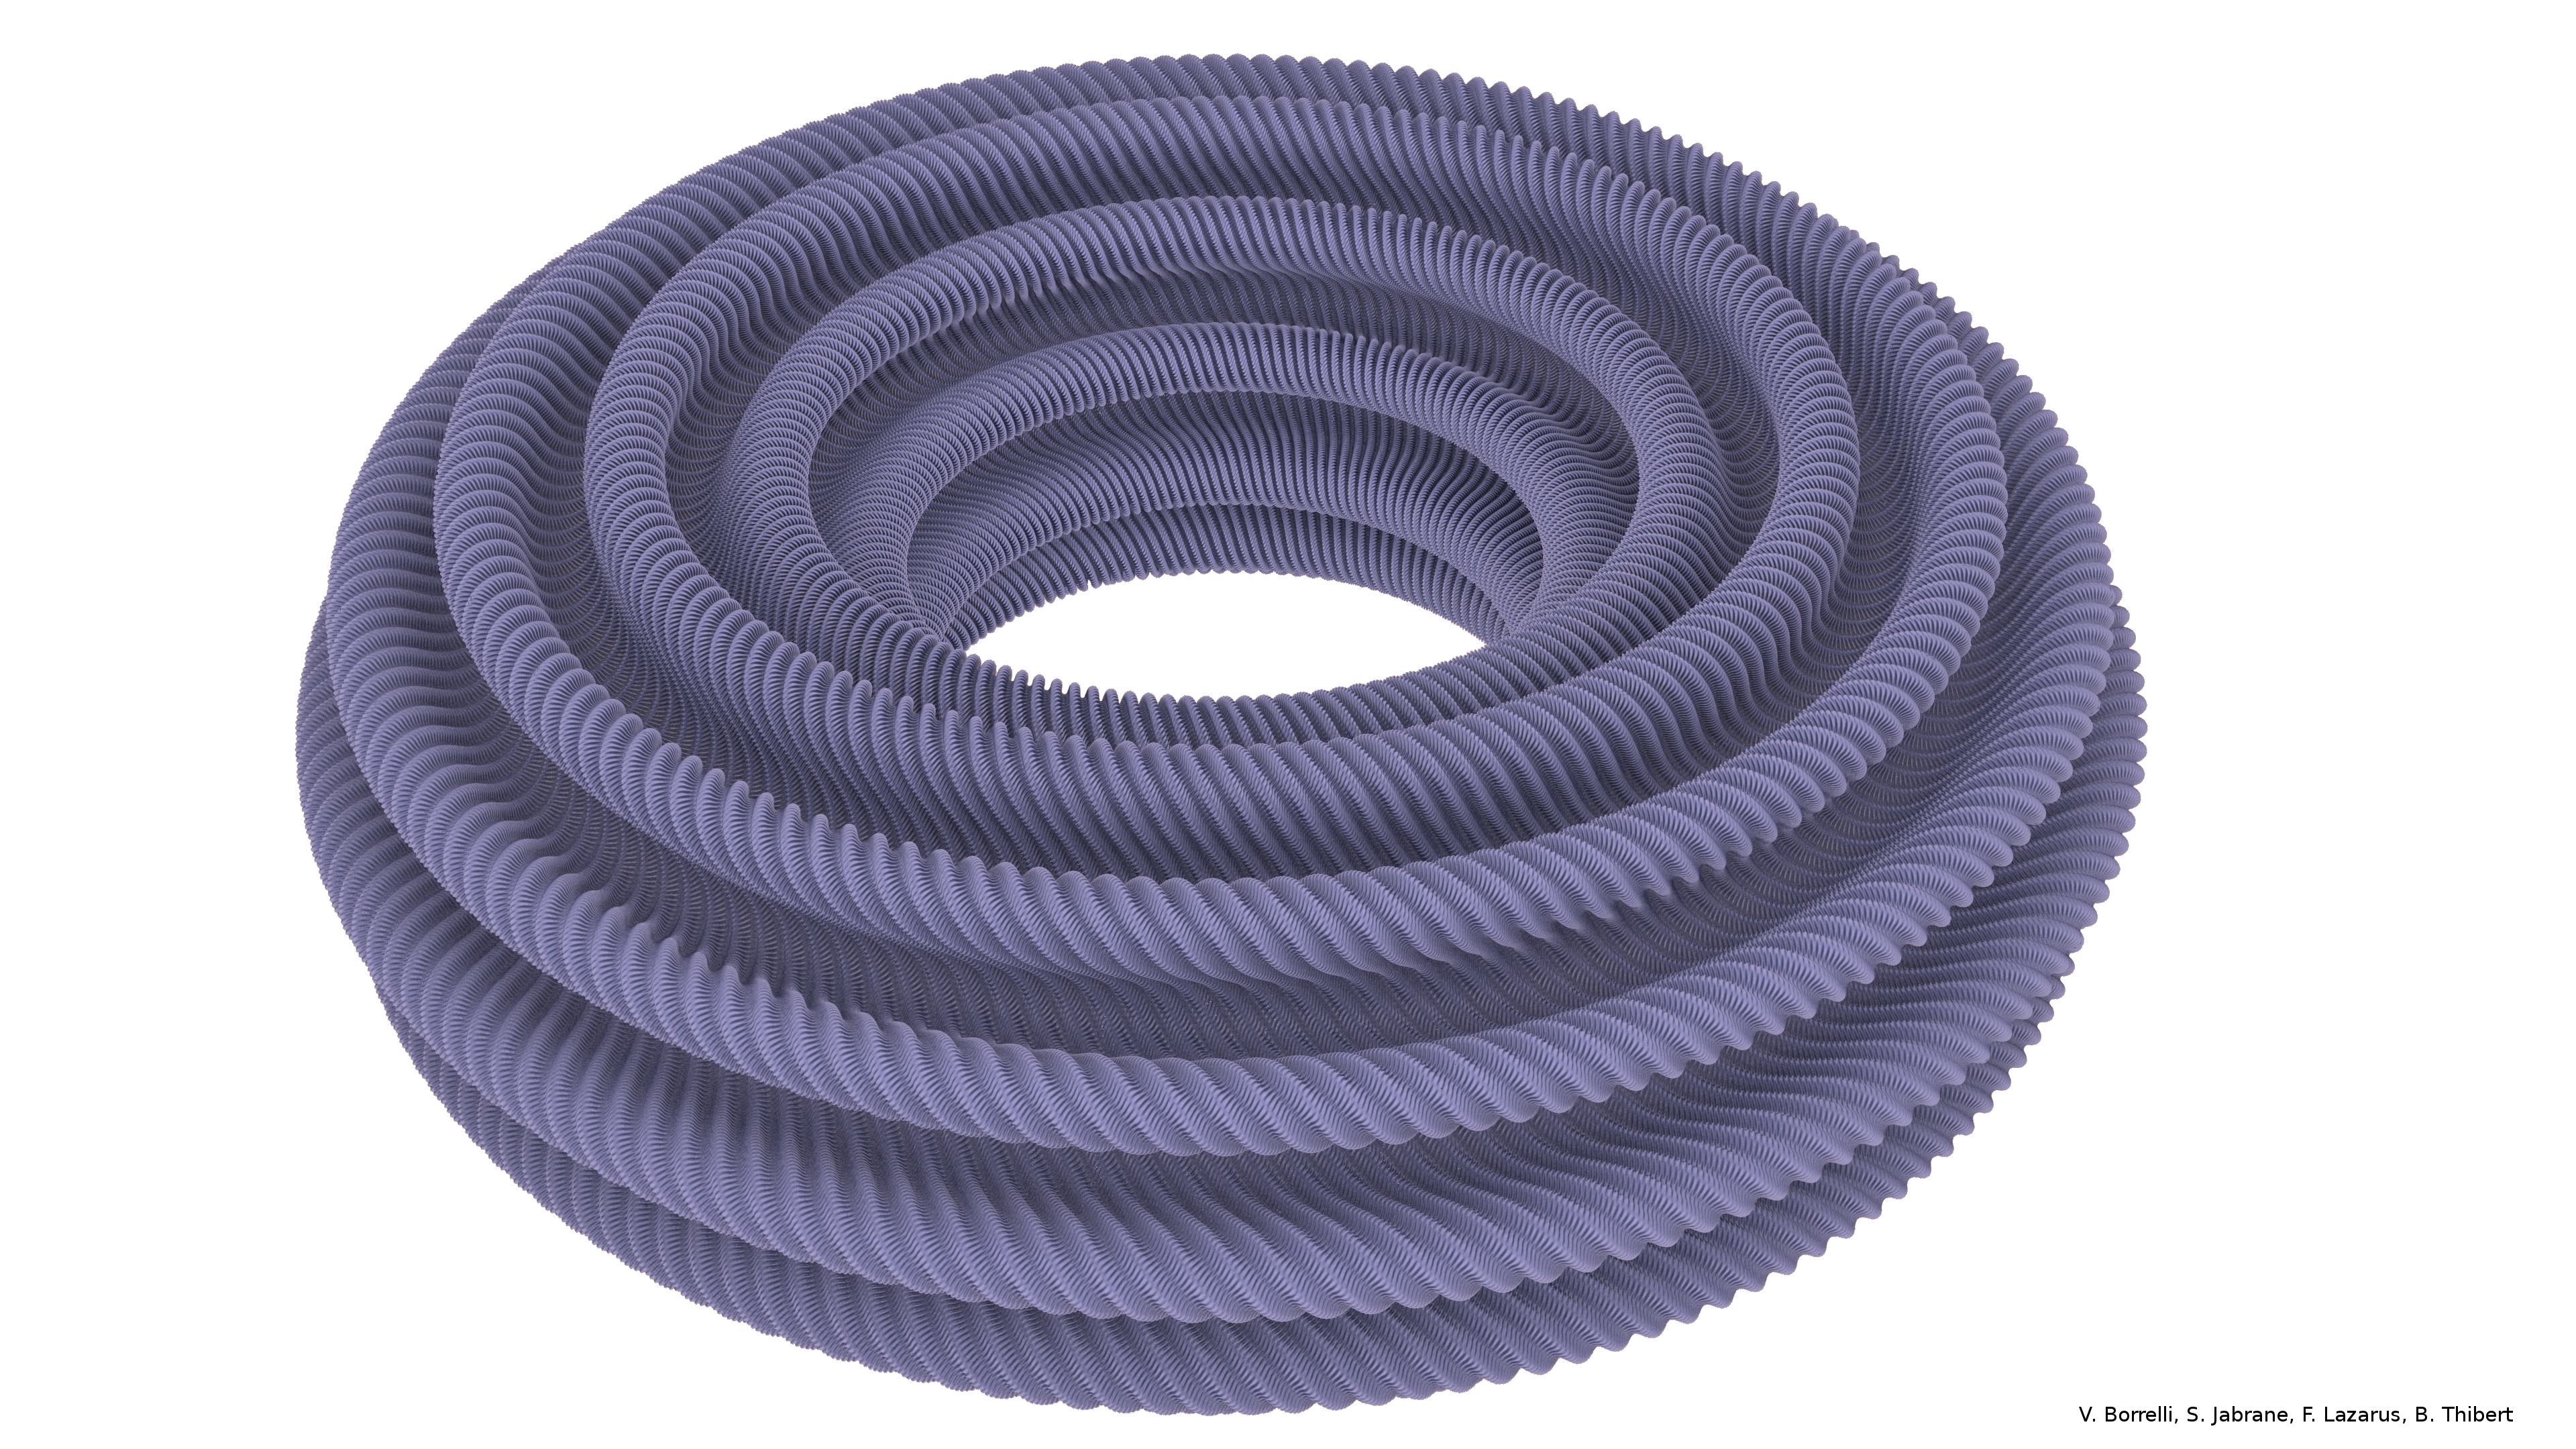
\includegraphics[width=0.8\textwidth]{4corrugations.jpg} % Nom de la imatge del tor
    \end{figure}
    
\end{frame}

\begin{frame}
    \frametitle{Conclusions}
    
    \begin{itemize}
        \item Hem explorat el contrast fonamental entre la \textbf{rigidesa} de la regularitat $C^\infty$ i la \textbf{flexibilitat} de la regularitat $C^1$ en el problema dels encabiments isomètrics.
        \pause
        \item La regularitat $C^\infty$ imposa restriccions fortes basades en la curvatura, com hem vist amb la impossibilitat d'encabir el tor pla o la mida mínima de la cinta de Möbius.
        \pause
        \item La regularitat $C^1$, en canvi, permet encabiments isomètrics en espais de dimensió sorprenentment baixa.
        \pause
        \item El mètode de Nash-Kuiper, basat en \textbf{corrugacions d'alta freqüència}, permet incrementar la mètrica d'un encabiment curt fins a fer-lo isomètric.
        \pause
        \item Aquest guany en flexibilitat, pagat amb una pèrdua de regularitat, porta a una geometria molt més rica i a objectes visualment complexos i contraintuïtius, com el tor pla que hem vist.
    \end{itemize}
    
\end{frame}

\begin{frame}
    \frametitle{Final}
    \begin{center}
        \Huge
        Gràcies per la vostra atenció.
        

    \end{center}
\end{frame}

\end{document}